%!TeX root=../../tcc.tex


\chapter{Par mais próximo cinético}\label{ch:par-mais-proximo-cinetico}

Considere o seguinte problema cinético.
São dados $n$ pontos movendo-se linearmente no plano.
Cada um destes pontos é representado por um par $(s_0, \vec{v})$ onde $s_0 = (x_0, y_0)$ é a sua
posição inicial e $\vec{v} = (v_x, v_y)$ um vetor velocidade.
A posição de um determinado ponto $p$ representado por $(s_0, \vec{v})$ num instante $t$, é
$s_p = (x_p, y_p) = (x_0, y_0) + t\cdot \vec{v}$.
Queremos num instante arbitrário $t \geq 0$ determinar um par $(p,q)$ dos $n$ pontos dados cuja
distância $d(p, q) = \sqrt{(x_p - x_q)^2 + (y_p - y_q)^2}$ é mínima.

Por exemplo, considere cinco pontos na coleção, representados na
Figura~\ref{fig:parestatico:exemplo}: $((1, 0), (2, 1))$, $((5, -1),
(-1, 2))$, $((0, 2), (1, -1))$, $((3, 2), (1, -2))$ e $((3, 1), (-1,
0))$.

\begin{figure}
    \centering
        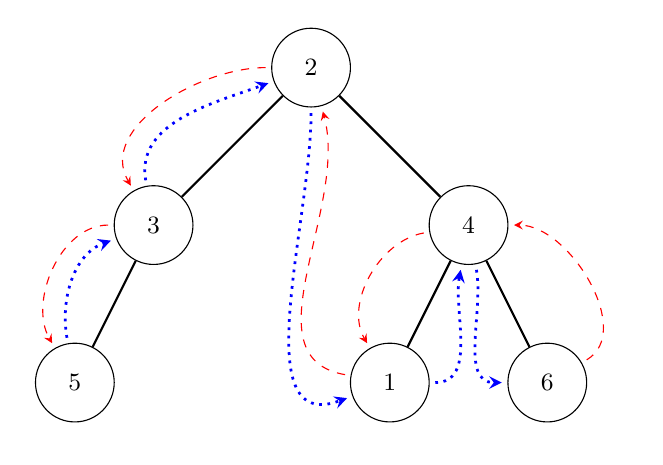
\begin{tikzpicture}[baseline=-2.25cm]
            \node[circle,draw,minimum size=1cm] (1) at (0,0)  {$2$};
            \node[circle,draw,minimum size=1cm] (2) at (-2,-2){$3$};
            \node[circle,draw,minimum size=1cm] (3) at (2,-2) {$4$};
            \node[circle,draw,minimum size=1cm] (4) at (-3,-4){$5$};
            \node[circle,draw,minimum size=1cm] (5) at (1,-4) {$1$};
            \node[circle,draw,minimum size=1cm] (6) at (3,-4) {$6$};
            % \node[label={7},circle,draw,minimum size=1cm] (7) at (3,-4) {$8$};
            % \node[label={8},circle,draw,minimum size=1cm] (8) at (-4,-6) {$4$};
            % \node[label={9},circle,draw,minimum size=1cm] (9) at (-2,-6) {$1$};
            \tikzstyle{filho}=[thick]
            \tikzstyle{pred}=[->, shorten >= 2pt, shorten <= 2pt,
                    dashed, >=stealth, red]
            \tikzstyle{sucessor}=[->, shorten >= 2pt, shorten <= 2pt,
                    dotted, >=stealth, blue, line width=0.35mm]
            % \tikzstyle{p4}=[->, shorten >= 2pt, shorten <= 2pt, dotted, >=stealth]
            \draw[filho] (1) -- (2);
            \draw[filho] (1) -- (3);
            \draw[filho] (2) -- (4);
            \draw[filho] (3) -- (5);
            \draw[filho] (3) -- (6);
            \draw[pred] (6) edge[out=30,in=0] (3);
            \draw[sucessor] (3) edge[out=280,in=180] (6);
            \draw[pred] (3) edge[out=190,in=120] (5);
            \draw[sucessor] (5) edge[out=0,in=260] (3);
            \draw[pred] (5) edge[out=170,in=285] (1);
            \draw[sucessor] (1) edge[out=270,in=200] (5);
            \draw[pred] (1) edge[out=180,in=120] (2);
            \draw[sucessor] (2) edge[out=100,in=200] (1);
            \draw[pred] (2) edge[out=180,in=120] (4);
            \draw[sucessor] (4) edge[out=100,in=200] (2);
        \end{tikzpicture}
        \qquad
        \qquad
        \qquad
        \begin{tabular}{|c|c|}
            \hline
            $i$ & $x_0$ \\
            \hline
            $1$ & $6$ \\

            $2$ & $3$ \\

            $3$ & $2$ \\

            $4$ & $7$ \\

            $5$ & $-2$ \\

            $6$ & $14$ \\
            \hline
        \end{tabular}
        \caption[Exemplo de estrutura da ABB]{Exemplo de árvore em
            que a ordem dos elementos, do menor para o maior no
            instante $\now = 0$, é $5 - 3 - 2 - 1 - 4 - 6$. Os
            apontadores para o elemento anterior são representados
            pelas setas vermelhas tracejadas e os apontadores para o
            elemento posterior são representados pelas setas azuis
            pontilhadas.}\label{fig:abb:exemplo}
\end{figure}

Queremos dar suporte às seguintes operações:
\begin{itemize}
    \item \textsc{advance}$(t)$ $\rightarrow$ avança o tempo corrente
    para $t$;
    \item \textsc{change}$(j, \vec{v})$ $\rightarrow$ altera a
    velocidade do ponto $j$ para $\vec{v}$;
    \item \textsc{query\textunderscore closest}$()$ $\rightarrow$
    devolve dois pontos que formam um par mais próximo no instante
    atual.
\end{itemize}

%!TeX root=./par.tex

\FloatBarrier
\section{Algoritmo Estático}

O algoritmo que será aqui apresentado foi proposto por Basch, Guibas
e Hershberger e admite uma boa cinetização, usando a ideia de linha
de varredura.

O algoritmo é baseado na ideia de dividir o plano, para cada ponto,
em seis cones iguais. Os cones são delimitados pela reta paralela ao
eixo $y$ que passa pelo ponto e pelas retas $x \pm 30^\circ$, isto
é, as retas que passam pelo ponto e formam $\pm 30^\circ$ com o eixo
$x$ como mostra a figura \ref{fig:parestatico:cones}.

\begin{figure}
    \centering
    \begin{tikzpicture}[thick]
        \draw (0, -3) -- (0, 3) node[anchor=north west] {$y$};
        \draw (-3, 1.7302) -- (3, -1.7302)
            node[anchor=north west] {$x - 30^\circ$};
        \draw (-3, -1.7302) -- (3, 1.7302)
            node[anchor=south west] {$x + 30^\circ$};
        \node[label=250:$p$] (p) at (0, 0) {\textbullet};
    \end{tikzpicture}
    \caption{A reta paralela ao eixo $y$ que passa por
    $p$ e as retas $x \pm 30^\circ$.}
    \label{fig:parestatico:cones}
\end{figure}

Tendo dividido o plano em cones, a ideia é achar o ponto mais próximo de $p$
dentro de cada um desses cones. Se assim o fizermos para todos os pontos, um
desses pares possui a menor distância entre si e será o par mais próximo que
buscamos.

Se $(p, q)$ formam um par mais próximo, então $(q, p)$ também serão um par
mais próximo, na verdade, serão o mesmo par. Dessa maneira, não precisamos
dos seis cones para buscar os pares, somente de três deles. Para uma
varredura da direita para a esquerda, apenas buscaremos os pares mais
próximos nos três cones à direita de p.

Vamos começar analisando o cone cujo eixo central é paralelo ao eixo $x$.
Chamaremos esse cone de \textit{dominância de p} e o representaremos por
$\Dom(p)$. Consideraremos que um ponto em cima da linha $x + 30^\circ$
pertence a $\Dom(p)$ e um ponto em cima de $x - 30^\circ$ não pertence a
$\Dom(p)$ como mostra a figura \ref{fig:parestatico:dominancia}. O mesmo
algoritmo poderá ser aplicado aos outros dois cones se rotacionarmos o
sistema de coordenadas~$\pm 60^\circ$.

\begin{figure}
    \centering
    \begin{tikzpicture}[thick]
        % \draw (0, -3) -- (0, 3) node[anchor=north west] {$y$};
        \draw (0, 0) -- (4, 2.309);
        \draw[dashed] (0, 0) -- (4, -2.309);
        \draw (0, 0) circle (2pt) node[label=250:$p$] {};
        \node[label=0:$q$] (q) at (1, 0) {\textbullet};
        \node[label=250:$r$] (r) at (3, 1.73) {\textbullet};
        \draw (3, -1.73) circle (2pt) node[label=250:$s$] {};
        % \node[label=250:$s$] (s) at (3, -1.73);
    \end{tikzpicture}
    \caption{Os pontos $q$ e $r$ pertencem a $Dom(p)$,
    mas o ponto $s$ não.}
    \label{fig:parestatico:dominancia}
\end{figure}

Definiremos como $\Maxima(p)$ o conjunto dos pontos à direita de $p$ que não
pertencem a \textit{dominância} de nenhum ponto à direita de $p$. Isso nos
permite definir o conjunto de \textit{candidatos} de $p$ representado por
$\Cands(p)$: $\Cands(p) = \Dom(p) \cap \Maxima(p)$, ou seja, os
\textit{candidatos} de $p$ são aqueles pontos à direita de $p$ que não
pertencem a \textit{dominância} de nenhum ponto à direita de $p$ e pertencem
a \textit{dominância} de $p$. Chamaremos o ponto de $\Maxima$ de menor
ordenada que está acima de $\Dom(p)$ de $\up(p)$ e chamaremos o ponto de
$\Maxima$ de maior ordenada que está abaixo de $\Dom(p)$ de $\low(p)$. Caso
não existam tais pontos $\up(p)$ e $\low(p)$ são \textit{NULL}. Os pontos
estritamente entre $\low(p)$ e $\up(p)$ são justamente os de $\Cands(p)$.
Dentre os \textit{candidatos} de $p$, chamaremos o ponto com menor
coordenada $x$ de $lcand(p)$. A figura
\ref{fig:parestatico:conjuntos}
mostra um exemplo dos conjuntos definidos.

\begin{figure}
    \centering
    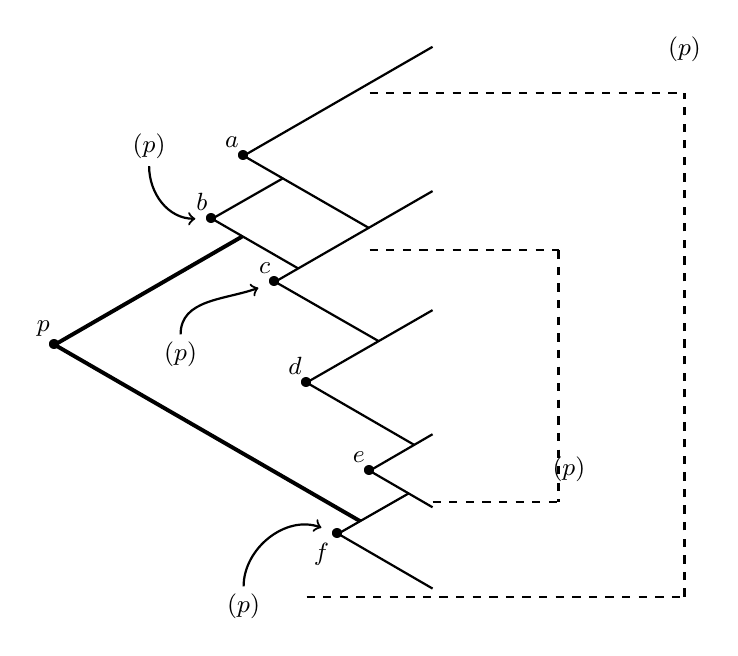
\begin{tikzpicture}[thick, scale=0.8]
        \node[label={[label distance = -3mm]160:$p$}]
            at (0.00, 0.00) {\textbullet};
        \node[label={[label distance = -3mm]160:$a$}]
            (a) at (3.00, 3.00) {\textbullet};
        \node[label={[label distance = -3mm]160:$b$}]
            (b) at (2.50, 2.00) {\textbullet};
        \node[label={[label distance = -3mm]160:$c$}]
            (c) at (3.50, 1.00) {\textbullet};
        \node[label={[label distance = -3mm]160:$d$}]
            at (4.00, -0.60) {\textbullet};
        \node[label={[label distance = -3mm]160:$e$}]
            at (5.00, -2.00) {\textbullet};
        \node[label={[label distance = -3mm]220:$f$}]
            (f) at (4.50, -3.00) {\textbullet};

        % e cone
        \draw (5.00, -2.00) -- (6.00, -2.58);
        \draw (5.00, -2.00) -- (6.00, -1.42);
        % f cone
        \draw (4.50, -3.00) -- (6.00, -3.87);
        \draw (4.50, -3.00) -- (5.62, -2.36);
        % d cone
        \draw (4.00, -0.60) -- (5.71, -1.59);
        \draw (4.00, -0.60) -- (6.00, 0.55);
        % c cone
        \draw (3.50, 1.00) -- (5.14, 0.06);
        \draw (3.50, 1.00) -- (6.00, 2.44);
        % a cone
        \draw (3.00, 3.00) -- (4.98, 1.86);
        \draw (3.00, 3.00) -- (6.00, 4.73);
        % b cone
        \draw (2.50, 2.00) -- (3.87, 1.21);
        \draw (2.50, 2.00) -- (3.62, 2.64);
        % p cone
        \draw[line width = 0.5mm] (0.00, 0.00) -- (4.85, -2.80);
        \draw[line width = 0.5mm] (0.00, 0.00) -- (2.98, 1.72);

        \draw[dashed] (6,-2.5) -- (8, -2.5)
            node[anchor=west, label=90:$\Cands(p)$] {};
        \draw[dashed] (8, 1.5) -- (8, -2.5);
        \draw[dashed] (5,1.5) -- (8, 1.5);

        \draw[dashed] (4, -4) -- (10, -4);
        \draw[dashed] (10, -4) -- (10, 4);
        \draw[dashed] (5, 4) -- (10, 4)
            node[anchor=south, label=$\Maxima(p)$] {};

        \node[label={[label distance = -3mm]270:$\low(p)$}]
            (low) at (3, -4) {};
        \draw[->] (low) edge[out=90,in=160] (f);

        \node[label={[label distance = -3mm]270:$\lcand(p)$}]
            (lc) at (2, 0) {};
        \draw[->] (lc) edge[out=90,in=200] (c);

        \node[label={[label distance = -3mm]90:$\up(p)$}]
            (up) at (1.5, 3) {};
        \draw[->] (up) edge[out=270,in=180] (b);
    \end{tikzpicture}
    \caption{Os pontos $c$, $d$ e $e$ pertencem a $\Cands(p)$, e todos os
    pontos exceto $p$ pertencem a $\Maxima(p)$. O ponto $b$ é $\up(p)$ e o
    ponto $f$ é $\low(p)$. O ponto $c$ é $\lcand(p)$.}
    \label{fig:parestatico:conjuntos}
\end{figure}

Consideraremos apenas os pares $(p, \lcand(p))$ como possíveis candidatos a
par mais próximo. Caso, para algum $p$, mais de um ponto atenda à condição
de ser $\lcand(p)$ poderemos escolher qualquer um deles como $\lcand(p)$,
pois, em um caso que há mais de um possível $\lcand(p)$, esses pontos
formarão um par mais próximo entre si do que o par $(p, \lcand(p))$, como
por exemplo na figura \ref{fig:parestatico:lcands}.
\begin{figure}
    \centering
    \begin{tikzpicture}[thick]
        % \draw (0, -3) -- (0, 3) node[anchor=north west] {$y$};
        \draw (0, 0) -- (4, 2.309);
        \draw[dashed] (0, 0) -- (4, -2.309);
        \node[label=250:$p$] (p) at (0, 0) {\textbullet};
        \node[label=0:$q$] (q) at (4, -1) {\textbullet};
        \node[label=250:$r$] (r) at (4, 1) {\textbullet};
        \draw[dotted] (4, -1) -- (4, 1);
        \draw[dotted] (0, 0) -- (r);
        \draw[dotted] (0, 0) -- (q);
    \end{tikzpicture}
    \caption{A distância de $r$ até $q$ é menor do que a
    distância $p$ até $r$ e do que a distância $p$ até $q$.}
    \label{fig:parestatico:lcands}
\end{figure}

O algoritmo \ref{parestatico:horizontal} descreve a sequência de operações a
serem feitas para achar o par mais próximo em alguma das ordens $(-60^\circ,
0^\circ, 60^\circ)$ representadas pelo ângulo $\theta$, dado em radianos.
Antes da rotina ser chamada os pontos devem ser ordenados de acordo com a
sua coordenada $x$. No algoritmo, $a$ e $b$ são os pontos que representam o
par mais próximo. Se $p$ ou $q$ são nulos, $d(p,q)$ retorna $+\infty$.

A cada iteração do algoritmo \ref{parestatico:horizontal}, $\Maxima$ é igual
a $\Maxima(p)$. Na nossa implementação, $\Maxima$ estará armazenado em uma
árvore binária de busca, mais especificamente em uma \textit{splay tree}
cuja chave é a coordenada $y$ dos pontos. Com isso, podemos buscar por
$\up(p)$ e $\low(p)$ em tempo logarítmico, bem como podemos retirar
$\Cands(p)$ de $\Maxima$ em tempo logarítmico, isto é, atualizar $\Maxima$
de maneira que $\Maxima = \Maxima \setminus \Cands(p)$.

\begin{algorithm}[H]
    \caption{Função \textsc{closest\_pair}$(p, n, \theta)$.}
    \label{parestatico:horizontal}
\begin{algorithmic}[1]
    \Function{closest\_pair}{$p, n, \theta$}
        \State $(a,b) \leftarrow (NULL, NULL)$
        \State \Call{heapsort}{$p, n, \theta$} \Comment{$p.x[1] > \cdots > p.x[n]$}
        \State $\Maxima \leftarrow \varnothing$
        \For{$i \leftarrow 1\To n$}
            \State $\Cands \leftarrow \Maxima\cap \Dom(p_i)$
            \State $\Maxima \leftarrow (\Maxima \setminus \Cands) \cup \lk p_i\rk$
            \State $\lcand \leftarrow \Call{min\_x}{\Cands}$
            \If{$d(p_i, \lcand) < d(a, b)$}
                \State $(a, b) \leftarrow (p_i, \lcand)$
            \EndIf
        \EndFor
        \State \Return{$(a, b)$}
    \EndFunction
\end{algorithmic}
\end{algorithm}

Para descrever a implementação do algoritmo, já considerando as versões
rotacionadas dele, iremos antes precisar estabelecer os nomes das variáveis
e rotinas auxiliares utilizadas. São elas:
\begin{enumerate}
    \item $n$: o número de pontos dados;
    \item \textit{point}: um ponto com os seguintes atributos:
    \begin{enumerate}
        \item $x$: coordenada $x$ do ponto;
        \item $y$: coordenada $y$ do ponto.
    \end{enumerate}
    \item \raiz: raiz da splay tree;
    \item \no: objeto que compõe a árvore de busca binária,
    atributos:
    \begin{enumerate}
        \item \esq$:$ aponta para a raiz da subárvore esquerda do nó. A
        subárvore esquerda é composta apenas por pontos que possuem
        \textit{key}~com menor ordenada que a \textit{key}~do nó;
        \item \dir$:$ aponta para a raiz da subárvore direita do nó. A
        subárvore direita é composta apenas por pontos que possuem
        \textit{key}~com ordenada maior ou igual que a \textit{key}~do nó;
        \item \pai$:$ aponta para o nó que é pai deste nó;
        \item \textit{key}$:$ aponta para um ponto.
    \end{enumerate}
    \item \angulo: ângulo de rotação do sistema de coordenadas;
    \item \pontos: vetor de $n$ posições que guarda os pontos;
    \item \textsc{getX}$(p) \rightarrow$ retorna a coordenada $x$
    de um ponto $p$ baseada no ângulo de rotação \angulo;
    \item \textsc{getY}$(p) \rightarrow$ retorna a coordenada $y$
    de um ponto $p$ baseada no ângulo de rotação \angulo;
    \item \textsc{heapsort}$() \rightarrow$ ordena o vetor \pontos,
    utilizando o algoritmo \textit{heapsort}, de acordo com a
    coordenada $x$ de cada ponto cujo valor é retornado
    pela rotina \textsc{getX}$(p)$.
\end{enumerate}

Para um ponto $(r, \phi)$ em coordenadas polares $x = rcos(\phi)$
e $y = rsen(\phi)$.

Rotacionar o sistema de coordenadas por $\theta$ é o mesmo que
transformar $\phi$ em $\phi - \theta$, veja a figura
\ref{fig:parestatico:rotacao}. Isso significa que agora as novas
coordenadas são descritas como:
\begin{align*}
    x^* & = rcos(\phi - \theta) = rcos(\phi)cos(\theta)
    + rsen(\phi)sen(\theta) = xcos(\theta) + ysen(\theta) \\
    y^* & = rsen(\phi - \theta) = rsen(\phi)cos(\theta)
    - rcos(\phi)sen(\theta) = ycos(\theta) - xsen(\theta)
\end{align*}
Os valores $x^*$ e $y^*$ são os valores, respectivamente,
retornados por \textsc{getX}$(p)$ e \textsc{getY}$(p)$ para
$\theta = \angulo$.

\begin{figure}
    \centering
    \begin{tikzpicture}[thick]
        \coordinate (a) at (0, 0);
        \coordinate (b) at (4, 0);
        \coordinate (c) at (2.828, 2.828);
        \coordinate (p) at (1, 2);
        \draw[thick,->] (0,0) -- (4,0)
            node[anchor=north west] {$x$};
        \draw[thick,->] (0,0) -- (0,4)
            node[anchor=south east] {$y$};
        \draw[thick,->, dashed] (0,0) -- (2.828,2.828)
            node[anchor=north west] {$x'$};
        \draw[thick,->, dashed] (0,0) -- (-2.828,2.828)
            node[anchor=south east] {$y'$};
        \pic [draw, angle radius = 0.5cm] {angle = b--a--c};
        \node[anchor=west, label={[label distance = 0mm]180:$\theta$}]
            (angl) at (1, 0.3) {};
        \node[label=90:$p$] at (p) {\textbullet};
        \draw[dashed,->] (a) -- node[above] {$r$} (p);
        \pic [draw, angle radius = 1cm] {angle = b--a--p};
        \node[anchor=west, label={[label distance = -3mm]180:$\phi$}]
            (angp) at (1.2, 0.7) {};
    \end{tikzpicture}
    \caption{O ponto $p$ está numa inclinação de $\phi - \theta$ graus
    em relação a reta que passa pela origem e por $x'$.}
    \label{fig:parestatico:rotacao}
\end{figure}

A interface da \textit{splay tree}, cuja chave é a
coordenada $y$ do ponto, contará com as seguintes operações além
das usuais:
\begin{enumerate}
    % \item \textsc{insert}$(p)\rightarrow$ insere o ponto $p$ na
    % \textit{splay tree} e chama $\textsc{splay}(x)$ para o nó $x$
    % cuja chave é $p$;
    \item \textsc{successor}$(p) \rightarrow$ busca pelo nó
    cuja chave é $\up(p)$ na \textit{splay tree}.
    Esse nó corresponde ao sucessor de $p$ na árvore;
    \item \textsc{predecessor}$(p) \rightarrow$ busca pelo nó cuja chave é $low(p)$ na \textit{splay tree}. Esse nó corresponde ao predecessor de $p$ na árvore;
    % \item \textsc{splay}$(x) \rightarrow$ dá um \textit{splay} no nó $x$;
    \item \textsc{lcand}$(p) \rightarrow$ calcula $\Cands(p)$, remove da
    \textit{splay tree} e determina $\lcand(p)$, que pode ser \textit{NULL};
    % \item \textsc{clearAll}$() \rightarrow$ remove todos os nós
    % da \textit{splay tree}.
\end{enumerate}

% As operações \textsc{insert}$(p)$, \textsc{splay}$(x)$ e
% \textsc{clearAll}$()$ não possuem nenhuma diferença quanto
% à sua implementação. São operações comuns de uma
% \textit{splay tree}. Portanto, focaremos em explicar as
% operações successor$(p)$, predecessor$(p)$ e lcand$(p)$.

No algoritmo \ref{parestatico:successor} e no algoritmo
\ref{parestatico:predecessor} a rotina checkLine$(p, q, \theta)$ retorna se o ponto
$q$ está à esquerda, sobre ou à direita da reta $r$. A reta $r$ é a reta que
passa por $p$ e faz um ângulo de $\theta$ radianos com o eixo $x$. Para $q$
à esquerda de $r$ o retorno é $1$, para $q$ sobre $r$ o retorno é $0$ e para
$q$ à direita de $r$, o retorno é $-1$.

O algoritmo \ref{parestatico:lcand} implementa a função \textsc{lcand}$(p)$.
Sabemos que $\lcand(p)$ é o elemento de $\Cands(p)$ com menor coordenada $x$
e que $\Cands(p)$ é limitado por $\low(p)$ e $\up(p)$. A ideia para retirar
$\Cands(p)$ da árvore é reorganizá-la de modo que $\low(p)$ seja a raiz e
$\up(p)$ o filho direito da raiz, dessa forma $\Cands(p)$ é a subárvore
esquerda do filho direito da raiz, veja a figura
\ref{fig:parestatico:loweup}. Nem sempre tal configuração é possível, mas o
algoritmo tratará dos casos de borda que são quando $\low(p)$, ou $\up(p)$,
ou ambos, não existem. A rotina \textsc{split}$(x)$ separa a subárvore de
raiz $x$ da \textit{splay tree} e retorna a raiz dessa nova árvore. A rotina
\textsc{min\_x}$(z)$ retorna o ponto com menor coordenada $x$ da árvore de
raiz~$z$.
\begin{figure}
    \centering
    \begin{tikzpicture}[thick]
        \tikzstyle{every node}=[font=\small]
        \node[every node,circle,draw, minimum size=1cm] (low) at (0, 0) {$l$};
        \node[every node,circle,draw, minimum size=1cm] (up) at (2, -2) {$u$};
        \node (esq) at (-2, -2) {$\gamma$};
        \node[every node] (esqesq) at (1, -4) {$\alpha$};
        \node[every node] (esqdir) at (3, -4) {$\beta$};
        \draw (low) -- (up);
        \draw (esqesq) -- (up);
        \draw (esqdir) -- (up);
        \draw (low) -- (esq);
    \end{tikzpicture}
    \caption{Na figura, $l$ é $low(p)$ e $u$ é $up(p)$. A subárvore $\alpha$ contém todos os pontos que estão entre $low(p)$ e $up(p)$ e, portanto, corresponde ao conjunto $Cands(p)$.}
    \label{fig:parestatico:loweup}
\end{figure}
\begin{algorithm}
    \caption{Função \textsc{successor}$(p)$.}
    \label{parestatico:successor}
\begin{algorithmic}[1]
    \Function{successor}{$p$}
        \State $x \leftarrow \raiz$
        \State $up \leftarrow NULL$
        \While{$x \neq NULL$}
            \State $y \leftarrow x$
            \If{$\Call{checkLine}{p, x.key, \pi/6}= -1$}
                \State $x \leftarrow x.right$
            \Else
                \State $up \leftarrow x$
                \State $x \leftarrow x.left$
            \EndIf
        \EndWhile
        \If{$y \neq NULL$} \Comment{dá \textsc{splay} no último nó visitado}
            \State \Call{splay}{$y$}
        \EndIf
        \State \Return{$up$}
    \EndFunction
\end{algorithmic}
\end{algorithm}

\begin{algorithm}
    \caption{Função \textsc{predecessor}$(p)$.}
    \label{parestatico:predecessor}
\begin{algorithmic}[1]
    \Function{predecessor}{$p$}
        \State $x \leftarrow \raiz$
        \State $low \leftarrow NULL$
        \While{$x \neq NULL$}
            \State $y \leftarrow x$
            \If{$\Call{checkLine}{p, x.key, -\pi/6}\leq 0$}
                \State $x \leftarrow x.left$
            \Else
                \State $low \leftarrow x$
                \State $x \leftarrow x.right$
            \EndIf
        \EndWhile
        \If{$y \neq NULL$} \Comment{dá \textsc{splay} no último nó visitado}
            \State \Call{splay}{$y$}
        \EndIf
        \State \Return{$low$}
    \EndFunction
\end{algorithmic}
\end{algorithm}

\begin{algorithm}
    \caption{Função lcand$(p)$.} \label{parestatico:lcand}
\begin{algorithmic}[1]
    \Function{lcand}{$p$}
        \State $r \leftarrow root$
        \State $low \leftarrow \Call{predecessor}{p}$
        \If{$low \neq NULL$}
            \State \Call{splay}{$low$}
            \State $r \leftarrow \Call{split}{low.right}$
        \EndIf
        \State $up \leftarrow \Call{successor}{p}$
        \If{$up \neq NULL$}
            \State $\Call{splay}{up}$
            \State $r \leftarrow \Call{split}{up.left}$
        \EndIf
        \If{$up \neq NULL$ \AND $low \neq NULL$}
            \State $low.right \leftarrow up$
            \State $up.parent \leftarrow low$
        \EndIf
        \State \Return{\Call{min\_x}{$r$}}
    \EndFunction
\end{algorithmic}
\end{algorithm}

O algoritmo \ref{parestatico:closest} implementa a função
\textsc{query\_closest} que retorna o par $(a,b)$ que possui distância
mínima em \pontos.

\begin{algorithm}
    \caption{Função \textsc{query\_closest}.} \label{parestatico:closest}
\begin{algorithmic}[1]
    \Function{query\_closest}{\null}
        \State $(m,n) \leftarrow (NULL, NULL)$
        \State \angulo~$\leftarrow -\frac{\pi}{3}$
        \While{\angulo~$\leq \frac{\pi}{3}$}
            \State \Call{heapsort}{$\pontos, n, \theta$} \Comment{$\pontos.x[1] > \cdots > \pontos.x[n]$}
            \For{$i \leftarrow 1$\To$n$}
                \State $p \leftarrow $~\pontos$[i]$
                \State $\lcand \leftarrow $ \Call{lcand}{$p$}
                \State \Call{insert}{$p$}
                \If{$d(p, \lcand) < d(a, b)$}
                    \State $(a, b) \leftarrow (p, \lcand)$
                \EndIf
            \EndFor
            \State \angulo~$\leftarrow$~\angulo~$ + \frac{\pi}{3}$
            \State \Call{clearAll}{\null} \Comment{esvazia a \textit{splay tree}}
        \EndWhile
        \State \Return{$(m,n)$}
    \EndFunction
\end{algorithmic}
\end{algorithm}

%!TeX root=./par.tex

\FloatBarrier


\section{Algoritmo cinético}\label{sec:algoritmo-cinetico}

Para ``cinetizar'' o algoritmo estático, utilizaremos certificados para assegurar que as nossas
estruturas permanecerão corretas.
Primeiramente, teremos os certificados das três \textit{listas ordenadas cinéticas}, conforme a
Seção~\ref{sec:heap-cinetico}, que guardarão a ordem dos pontos de acordo com os eixos $x$, $x +
60^\circ$ e $x - 60^\circ$.

Para garantir qual, dentre os pares $(p, \lcand(p))$, é o par mais próximo, usaremos um
\textit{torneio cinético com inserção e remoção}, conforme a Seção~\ref{subsec:torneio-insere-remove},
com respeito ao mínimo em vez de ao máximo.
Temos um total de $3n$ pares, pois consideraremos também os pares $(p, \lcand(p))$ em que
$\lcand(p)$ é nulo e os certificados destes serão $+\infty$.

Também precisaremos manter informação guardada para atualizar com eficiência mudanças provocadas
por trocas na ordem dos pontos em relação a um dos três eixos.
Por exemplo, uma troca na ordem dos pontos pode acarretar numa mudança nos conjuntos $\Cands(p)$ e
$\Cands(q)$.
Mudanças nesses conjuntos ocorrerão quando $q = \up(p)$, $q = \low(p)$ ou $q \in \Cands(p)$.
Portanto, para que consigamos manter $\lcand(p)$ de maneira eficiente, cada ponto terá três árvores
binárias de busca associadas a ele com os conjuntos $\Cands(p)$, $\Hits_{up}(p)$ e $\Hits_{low}(p)
$.
A árvore $\Cands(p)$ guarda os pontos que pertencem ao conjunto $\Cands(p)$ ordenados pela
coordenada $y$.
A árvore $\Hits_{up}(p)$ guarda os pontos $q$ tais que $\up(q) = p$, ordenados pela coordenada $x$.
Similarmente, a árvore $\Hits_{low}(p)$ guarda os pontos $q$ tais que $\low(q) = p$, ordenados
pela coordenada $x$.
Utilizaremos as árvores $\Cands(p)$, $\Hits_{up}(p)$ e $\Hits_{low}(p)$ para cada um dos eixos,
logo, para cada ponto $p$, haverão nove \textit{splay trees} no total.

Cada uma das nove árvores têm sua raiz apontando para o nó $p$, e cada nó das árvores aponta para
o seu nó pai.
Na árvore $\Cands(p)$, cada nó deve apontar para o descendente que contém o ponto mais à esquerda
na ordenação horizontal.
Na nossa implementação, as árvores serão \textit{splay trees}.
Essas estruturas contêm toda a informação necessária para que mantenhamos nossas estruturas
atualizadas e, consequentemente, o par mais próximo do conjunto.

Na implementação do algoritmo, inicialmente inserimos os pontos nas três listas ordenadas.
Uma vez que as listas estejam montadas, percorremos os pontos da direita para a esquerda
preenchendo as estruturas $\Cands(p)$, $\Hits_{up}(p)$ e $\Hits_{low}(p)$ para cada ponto $p$ e
para cada um dos eixos.
Esta etapa é feita da mesma forma que foi apresentada na seção sobre o algoritmo estático, a
Seção~\ref{sec:algoritmo-estatico}.

A medida que as estruturas $\Cands(p)$ são inicializadas, inserimos o par $(p, \lcand(p))$ no
torneio.
Quando todos os pares forem inseridos no torneio, realizamos as partidas e calculamos os
certificados.
O par $(p, q)$ da partida que possuir menor distância é considerado o vencedor.

Todos os certificados são colocados em uma fila de prioridade $Q$.
Os certificados inseridos na fila possuem quatro informações:
\begin{itemize}
    \item $t~\rightarrow$ instante de tempo em que o certificado
    expira.
    É utilizado como chave para a fila de prioridade.
    Desempates são tratados de maneira especial e serão explicados
    mais adiante;
    \item $p~\rightarrow$ um dos pontos envolvidos no evento
    representado pelo certificado.
    Caso seja um certificado de troca na ordenação, $p$ é o ponto mais à direita naquela ordenação;
    \item $q~\rightarrow$ o outro ponto envolvido no evento representado pelo certificado.
    Caso seja um certificado de troca na ordenação, $q$ é o ponto mais à esquerda naquela
    ordenação;
    \item tipo $ \rightarrow$ o tipo de evento que o certificado representa.
    Pode representar uma troca em uma das três ordenações, denominadas por \textit{H} (horizontal =
    $0^\circ$-ordem), \textit{U} (up = $+60^\circ$-ordem) e \textit{D} (down = $-60^\circ$-ordem) ou pode
    representar a vitória do par $(p, q)$ em uma partida do torneio.
\end{itemize}

\begin{figure}[H]
    \centering
    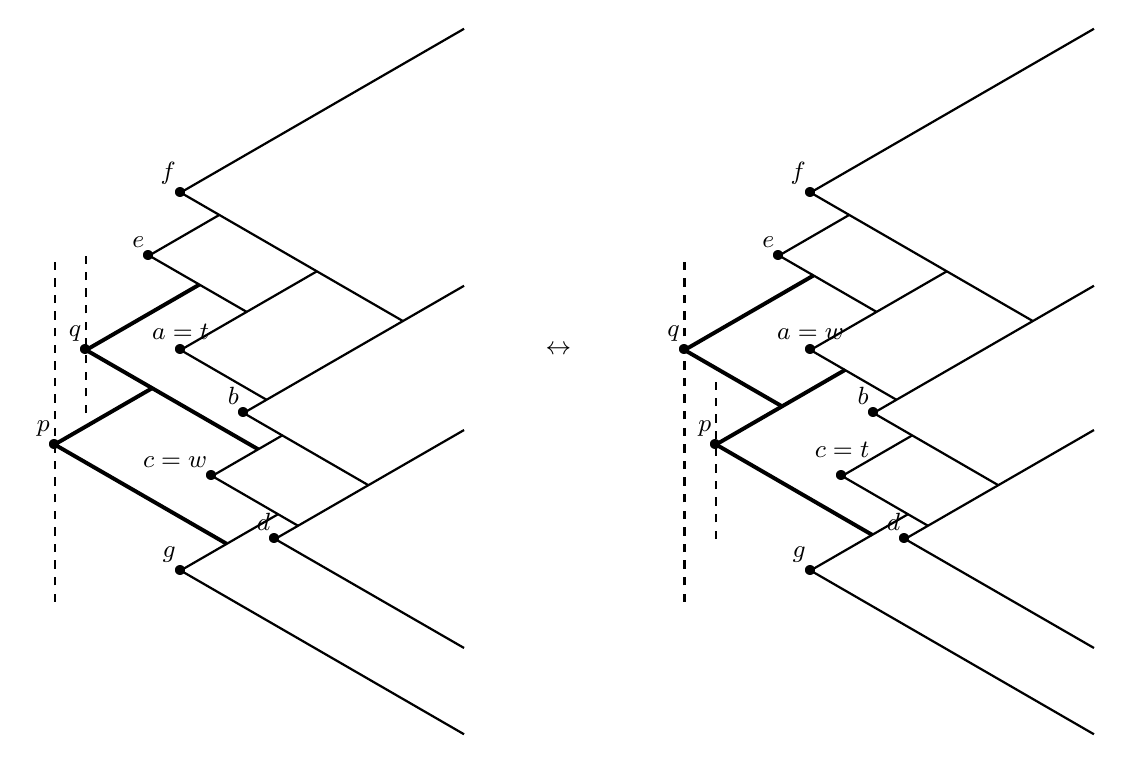
\begin{tikzpicture}[thick, scale=0.4]
        \node[label={[label distance = -3mm]160:$p$}] at
        (2.00, 2.00) {\textbullet};
        \node[label={[label distance = -3mm]160:$q$}] at
        (3.00, 5.00) {\textbullet};
        \node[label={[label distance = -2mm]90:$a = t$}] at
        (6.00, 5.00) {\textbullet};
        \node[label={[label distance = -3mm]160:$b$}] at
        (8.00, 3.00) {\textbullet};
        \node[label={[label distance = -3mm]160:$c = w$}] at
        (7.00, 1.00) {\textbullet};
        \node[label={[label distance = -3mm]160:$d$}] at
        (9.00, -1.00) {\textbullet};
        \node[label={[label distance = -3mm]160:$e$}] at
        (5.00, 8.00) {\textbullet};
        \node[label={[label distance = -3mm]160:$f$}] at
        (6.00, 10.00) {\textbullet};
        \node[label={[label distance = -3mm]160:$g$}] at
        (6.00, -2.00) {\textbullet};
        % d cone
        \draw (9.00, -1.00) -- (15.00, -4.46);
        \draw (9.00, -1.00) -- (15.00, 2.46);
        % b cone
        \draw (8.00, 3.00) -- (11.96, 0.71);
        \draw (8.00, 3.00) -- (15.00, 7.04);
        % c cone
        \draw (7.00, 1.00) -- (9.73, -0.58);
        \draw (7.00, 1.00) -- (9.23, 2.29);
        % f cone
        \draw (6.00, 10.00) -- (13.06, 5.92);
        \draw (6.00, 10.00) -- (15.00, 15.20);
        % g cone
        \draw (6.00, -2.00) -- (15.00, -7.20);
        \draw (6.00, -2.00) -- (9.10, -0.21);
        % a cone
        \draw (6.00, 5.00) -- (8.73, 3.42);
        \draw (6.00, 5.00) -- (10.33, 7.50);
        % e cone
        \draw (5.00, 8.00) -- (8.10, 6.21);
        \draw (5.00, 8.00) -- (7.23, 9.29);
        % q cone
        \draw[line width = 0.5mm] (3.00, 5.00) -- (8.46, 1.85);
        \draw[line width = 0.5mm] (3.00, 5.00) -- (6.60, 7.08);
        % p cone
        \draw[line width = 0.5mm] (2.00, 2.00) -- (7.46, -1.15);
        \draw[line width = 0.5mm] (2.00, 2.00) -- (5.10, 3.79);

        \draw[dashed] (2, -3) -- (2, 8);
        \draw[dashed] (3, 3) -- (3, 8);

        \node at (18, 5) {$ \leftrightarrow$};

        \node[label={[label distance = -3mm]160:$p$}] at
        (23.00, 2.00) {\textbullet};
        \node[label={[label distance = -3mm]160:$q$}] at
        (22.00, 5.00) {\textbullet};
        \node[label={[label distance = -2mm]90:$a = w$}] at
        (26.00, 5.00) {\textbullet};
        \node[label={[label distance = -3mm]160:$b$}] at
        (28.00, 3.00) {\textbullet};
        \node[label={[label distance = -1mm]90:$c = t$}] at
        (27.00, 1.00) {\textbullet};
        \node[label={[label distance = -3mm]160:$d$}] at
        (29.00, -1.00) {\textbullet};
        \node[label={[label distance = -3mm]160:$e$}] at
        (25.00, 8.00) {\textbullet};
        \node[label={[label distance = -3mm]160:$f$}] at
        (26.00, 10.00) {\textbullet};
        \node[label={[label distance = -3mm]160:$g$}] at
        (26.00, -2.00) {\textbullet};
        % d cone
        \draw (29.00, -1.00) -- (35.00, -4.46);
        \draw (29.00, -1.00) -- (35.00, 2.46);
        % b cone
        \draw (28.00, 3.00) -- (31.96, 0.71);
        \draw (28.00, 3.00) -- (35.00, 7.04);
        % c cone
        \draw (27.00, 1.00) -- (29.73, -0.58);
        \draw (27.00, 1.00) -- (29.23, 2.29);
        % f cone
        \draw (26.00, 10.00) -- (33.06, 5.92);
        \draw (26.00, 10.00) -- (35.00, 15.20);
        % g cone
        \draw (26.00, -2.00) -- (35.00, -7.20);
        \draw (26.00, -2.00) -- (29.10, -0.21);
        % a cone
        \draw (26.00, 5.00) -- (28.73, 3.42);
        \draw (26.00, 5.00) -- (30.33, 7.50);
        % e cone
        \draw (25.00, 8.00) -- (28.10, 6.21);
        \draw (25.00, 8.00) -- (27.23, 9.29);
        % p cone
        \draw[line width = 0.5mm] (23.00, 2.00) -- (27.96, -0.87);
        \draw[line width = 0.5mm] (23.00, 2.00) -- (27.10, 4.37);
        % q cone
        \draw[line width = 0.5mm] (22.00, 5.00) -- (25.10, 3.21);
        \draw[line width = 0.5mm] (22.00, 5.00) -- (26.10, 7.37);

        \draw[dashed] (22, -3) -- (22, 8);
        \draw[dashed] (23, -1) -- (23, 4);
    \end{tikzpicture}
    \caption{Da esquerda para a direita, o caso em que
        $p$ está em $\Hits_{up}(q)$. Da direita para a esquerda,
        o caso em que $q$ está em $\Hits_{low}(p)$.}
    \label{fig:parcinetico:eventohorizontalabaixo}
\end{figure}

Vamos agora falar de um evento em que ocorre uma mudança na ordem horizontal.
No primeiro caso, $p$ se encontra à esquerda e abaixo de $q$, veja a
Figura~\ref{fig:parcinetico:eventohorizontal}.
O caso em que $q$ está à esquerda de $p$ será tratado de maneira parecida.
O Algoritmo~\ref{alg:par-cinetico:eventohorizontal} implementa a sequência de operações referentes
a esse tipo de evento.

\begin{algorithm}[H]
    \caption{Função \textsc{horizontalEvent}.}
    \label{alg:par-cinetico:eventohorizontal}
    \begin{algorithmic}[1]
        \Function{horizontalEvent}{$p,q, dir$}
            \If{$q = \Call{owner}{p.\hitsup(dir)}$}
                \State \Call{horizontalEventLeft}{$p,q, dir$}
            \Else
                \If{$p = \Call{owner}{q.\hitslow(p, dir)}$}
                    \State \Call{horizontalEventRight}{$p,q, dir$}
                \EndIf
            \EndIf
            \State $v \leftarrow \Call{owner}{p.cands(dir)}$
            \State $v' \leftarrow \Call{owner}{q.cands(dir)}$
            \If{$v = v'$}
                \State \Call{updateLcand}{$v, dir$}
            \EndIf
        \EndFunction
    \end{algorithmic}
\end{algorithm}

Se $p$ está à esquerda de $q$ e em $\Hits_{up}(q)$, como demonstrado na
Figura~\ref{fig:parcinetico:eventohorizontal}, então parte de $\Cands(q)$ terá de passar
para $\Cands(p)$.
Além disso, também teremos alterações em $\Hits_{low}(q)$, $\Hits_{up}(q)$, $\Hits_{up}(t)$ e
$\Hits_{low}(w)$, onde $t = \up(p)$ após a troca de ordem entre os pontos e $w = \low(q)$ antes da
troca de ordem entre os pontos.
O Algoritmo~\ref{alg:par-cinetico:eventohorizontalcaso1} implementa a sequência de operações
necessárias para corrigir as estruturas afetadas pela troca.
A rotina \textsc{owner} acha em tempo logarítmico na quantidade de nós da árvore o ponto para o
qual a raiz aponta.
Os atributos $\hitsup$ e $\hitslow$ são apontadores para o nó do ponto na respectiva árvore da
direção especificada.
Por exemplo, $q.\hitsup(U)$ é o apontador para o nó de $q$ numa árvore $\Hits_{up}$ de algum
ponto, na direção \textsc{up}.
Se $p$ não está em $\Hits_{up}(q)$, então não haverão mudanças, veja a
Figura~\ref{fig:parcinetico:eventohorizontalabaixosemmudancas}.

Similarmente, se $q$ está em $\Hits_{low}(p)$, como demonstrado na
Figura~\ref{fig:parcinetico:eventohorizontal}, parte de $\Cands(p)$ passará a $\Cands(q)$.
Além disso, também teremos alterações em $\Hits_{low}(q)$, $\Hits_{up}(q)$, $\Hits_{up}(t)$ e
$\Hits_{low}(w)$, onde $t = \low(q)$ após a troca de ordem entre os pontos e $w = \up(p)$ antes da
troca de ordem entre os pontos.
O Algoritmo~\ref{alg:par-cinetico:eventohorizontalcaso2} implementa a sequência de operações
necessárias para corrigir as estruturas afetadas pela troca.
Se $q$ não está em $Hits_{low}(p)$, então não haverão mudanças, veja a
Figura~\ref{fig:parcinetico:eventohorizontalabaixosemmudancas}.

\begin{figure}[H]
    \centering
    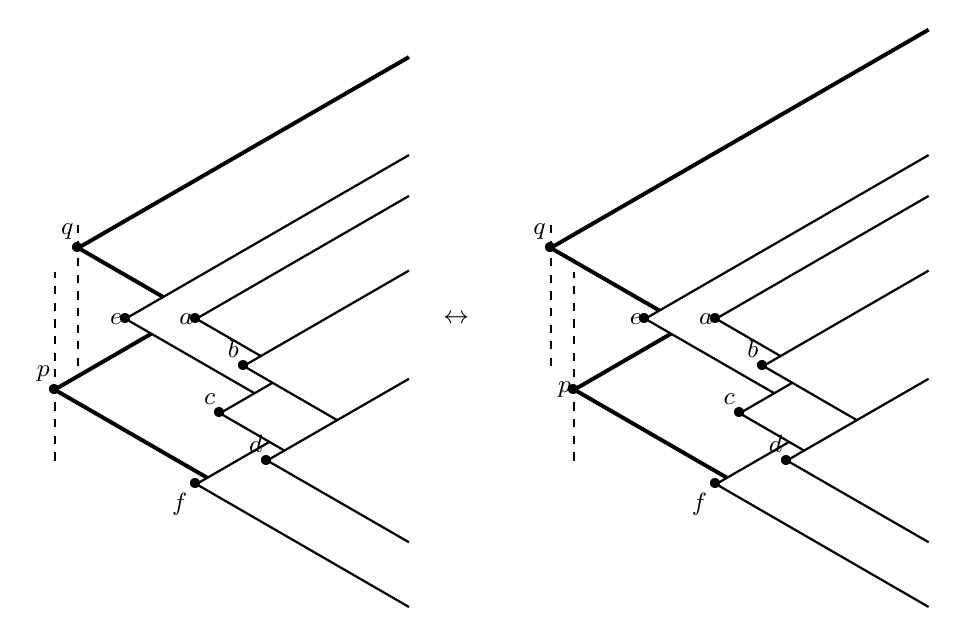
\begin{tikzpicture}[thick, scale=0.3]
        \node[label={[label distance = -3mm]160:$p$}] at
        (-1, 2.00) {\textbullet};
        \node[label={[label distance = -3mm]180:$e$}] at
        (2.00, 5.00) {\textbullet};
        \node[label={[label distance = -3mm]180:$a$}] at
        (5.00, 5.00) {\textbullet};
        \node[label={[label distance = -3mm]160:$b$}] at
        (7.00, 3.00) {\textbullet};
        \node[label={[label distance = -3mm]160:$c$}] at
        (6.00, 1.00) {\textbullet};
        \node[label={[label distance = -3mm]160:$d$}] at
        (8.00, -1.00) {\textbullet};
        \node[label={[label distance = -3mm]160:$q$}] at
        (0.00, 8.00) {\textbullet};
        \node[label={[label distance = -3mm]220:$f$}] at
        (5.00, -2.00) {\textbullet};

        % d cone
        \draw (8.00, -1.00) -- (14.00, -4.46);
        \draw (8.00, -1.00) -- (14.00, 2.46);
        % b cone
        \draw (7.00, 3.00) -- (10.96, 0.71);
        \draw (7.00, 3.00) -- (14.00, 7.04);
        % c cone
        \draw (6.00, 1.00) -- (8.73, -0.58);
        \draw (6.00, 1.00) -- (8.23, 2.29);
        % f cone
        \draw (5.00, -2.00) -- (14.00, -7.20);
        \draw (5.00, -2.00) -- (8.10, -0.21);
        % a cone
        \draw (5.00, 5.00) -- (7.73, 3.42);
        \draw (5.00, 5.00) -- (14.00, 10.20);
        % e cone
        \draw (2.00, 5.00) -- (7.46, 1.85);
        \draw (2.00, 5.00) -- (14.00, 11.93);
        % q cone
        \draw[line width = 0.5mm] (0.00, 8.00) -- (3.60, 5.92);
        \draw[line width = 0.5mm] (0.00, 8.00) -- (14.00, 16.08);
        % p cone
        \draw[line width = 0.5mm] (-1.00, 2.00) -- (5.46, -1.73);
        \draw[line width = 0.5mm] (-1.00, 2.00) -- (3.10, 4.37);

        \draw[dashed] (-1, -1) -- (-1, 7);
        \draw[dashed] (0, 3) -- (0, 9);

        \draw[dashed] (21, -1) -- (21, 7);
        \draw[dashed] (20, 3) -- (20, 9);

        \node at (16, 5) {$ \leftrightarrow$};

        \node[label={[label distance = -3mm]180:$p$}] at
        (21.00, 2.00) {\textbullet};
        \node[label={[label distance = -3mm]180:$e$}] at
        (24.00, 5.00) {\textbullet};
        \node[label={[label distance = -3mm]180:$a$}] at
        (27.00, 5.00) {\textbullet};
        \node[label={[label distance = -3mm]160:$b$}] at
        (29.00, 3.00) {\textbullet};
        \node[label={[label distance = -3mm]160:$c$}] at
        (28.00, 1.00) {\textbullet};
        \node[label={[label distance = -3mm]160:$d$}] at
        (30.00, -1.00) {\textbullet};
        \node[label={[label distance = -3mm]160:$q$}] at
        (20.00, 8.00) {\textbullet};
        \node[label={[label distance = -3mm]220:$f$}] at
        (27.00, -2.00) {\textbullet};

        % d cone
        \draw (30.00, -1.00) -- (36.00, -4.46);
        \draw (30.00, -1.00) -- (36.00, 2.46);
        % b cone
        \draw (29.00, 3.00) -- (32.96, 0.71);
        \draw (29.00, 3.00) -- (36.00, 7.04);
        % c cone
        \draw (28.00, 1.00) -- (30.73, -0.58);
        \draw (28.00, 1.00) -- (30.23, 2.29);
        % f cone
        \draw (27.00, -2.00) -- (36.00, -7.20);
        \draw (27.00, -2.00) -- (30.10, -0.21);
        % a cone
        \draw (27.00, 5.00) -- (29.73, 3.42);
        \draw (27.00, 5.00) -- (36.00, 10.20);
        % e cone
        \draw (24.00, 5.00) -- (29.46, 1.85);
        \draw (24.00, 5.00) -- (36.00, 11.93);
        % p cone
        \draw[line width = 0.5mm] (21.00, 2.00) -- (27.46, -1.73);
        \draw[line width = 0.5mm] (21.00, 2.00) -- (25.10, 4.37);
        % q cone
        \draw[line width = 0.5mm] (20.00, 8.00) -- (24.60, 5.35);
        \draw[line width = 0.5mm] (20.00, 8.00) -- (36.00, 17.24);
    \end{tikzpicture}
    \caption[Exemplo de evento \textsc{horizontal} em que nada acontece]{Se $p$ não está em $\Hits_{up}(q)$, ou se
    $q$ não está em $\Hits_{low}(p)$, nada acontece.}
    \label{fig:parcinetico:eventohorizontalabaixosemmudancas}
\end{figure}

\begin{algorithm}[H]
    \caption[Algoritmo \textsc{horizontalEventLeft} do par mais próximo cinético]{Função \textsc{horizontalEventLeft}.}
    \label{alg:par-cinetico:eventohorizontalcaso1}
    \begin{algorithmic}[1]
        \Function{horizontalEventLeft}{$p, q, dir$}
            \State $t \leftarrow$ \Call{predecessor}{$p, \Cands(q, dir), U$}
            \If{$t = \nnull$}
                \State $t \leftarrow$ \Call{owner}{$q.\hitsup(dir)$}
            \EndIf
            \State $newCands \leftarrow$ \Call{split}{$\nnull, t, \Cands(q,
            dir)$}
            \State \Call{join}{$\Cands(p, dir), newCands$}
            \State \Call{delete}{$p, \Hits_{up}(q, dir)$}
            \If{$t \neq \nnull$}
                \State \Call{insert}{$p, \Hits_{up}(t, dir)$}
            \EndIf

            \State $w \leftarrow \Call{owner}{q.\hitslow(dir)}$

            \If{$w \neq \nnull$}
                \State \Call{delete}{$q, \Hits_{low}(w, dir)$}
            \EndIf

            \State \Call{insert}{$q, \Hits_{low}(p, dir)$}
        \EndFunction
    \end{algorithmic}
\end{algorithm}

\begin{algorithm}[H]
    \caption[Algoritmo \textsc{horizontalEventRight} do par mais próximo cinético]{Função \textsc{horizontalEventRight}.}
    \label{alg:par-cinetico:eventohorizontalcaso2}
    \begin{algorithmic}[1]
        \Function{horizontalEventRight}{$p, q, dir$}
            \State $t \leftarrow$ \Call{predecessor}{$q, \Cands(p, dir), D$}
            \If{$t = \nnull$}
                \State $t \leftarrow$ \Call{owner}{$p.\hitslow(dir)$}
            \EndIf
            \State $newCands \leftarrow \Call{split}{t, \nnull, \Cands(p,
            dir)}$
            \State \Call{join}{$\Cands(q, dir), newCands$}
            \State \Call{delete}{$q, \Hits_{low}(p, dir)$}
            \If{$t \neq \nnull$}
                \State \Call{insert}{$q, \Hits_{low}(t, dir)$}
            \EndIf
            \State $w \leftarrow \Call{owner}{p.\hitsup(dir)}$
            \If{$w \neq \nnull$}
                \State \Call{delete}{$p, \Hits_{up}(w, dir)$}
            \EndIf
            \State \Call{insert}{$p, \Hits_{up}(q, dir)$}
        \EndFunction
    \end{algorithmic}
\end{algorithm}

Na mudança horizontal também precisamos nos preocupar com a possível troca de um
$\lcand$, se $p$ e $q$ estão em $\Cands$ de um mesmo ponto $v$, como verificado na linha $9$ do
Algoritmo~\ref{alg:par-cinetico:eventohorizontal}.

\begin{figure}[H]
    \centering
    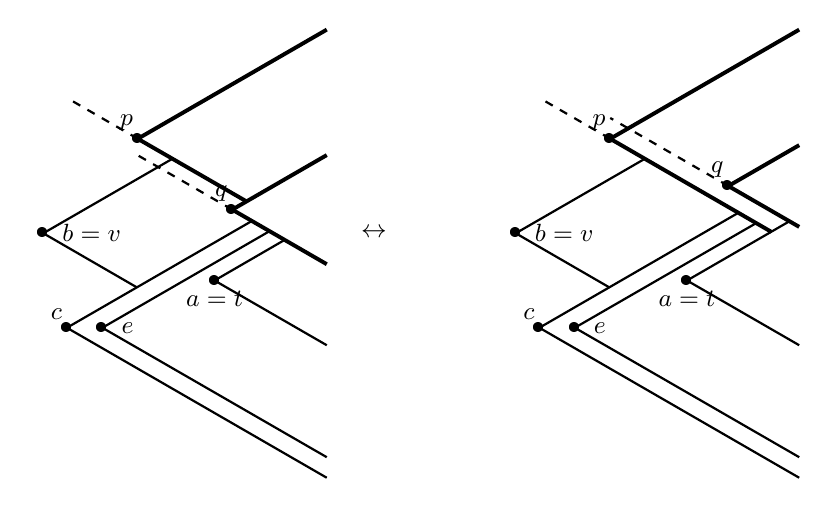
\begin{tikzpicture}[thick, scale=0.3]
        \node[label={[label distance = -3mm]160:$p$}] at
        (2.00, 4.00) {\textbullet};
        \node[label={[label distance = -3mm]160:$q$}] at
        (6.00, 1.00) {\textbullet};
        \node[label={[label distance = -2mm]270:$a = t$}] at
        (5.25, -2.00) {\textbullet};
        % \node[label={[label distance = -3mm]160:$b$}] at (-5.00, 0.00) {\textbullet};
        \node[label={[label distance = -3mm]160:$c$}] at
        (-1.00, -4.00) {\textbullet};
        \node[label={[label distance = -1mm]0:$b = v$}] at
        (-2.00, 0.00) {\textbullet};
        \node[label={[label distance = -1mm]0:$e$}] at
        (0.50, -4.00) {\textbullet};

        % q cone
        \draw[line width = 0.5mm] (6.00, 1.00) -- (10.00, -1.31);
        \draw[line width = 0.5mm] (6.00, 1.00) -- (10.00, 3.31);
        % a cone
        \draw (5.25, -2.00) -- (10.00, -4.74);
        \draw (5.25, -2.00) -- (8.22, -0.28);
        % p cone
        \draw[line width = 0.5mm] (2.00, 4.00) -- (6.60, 1.35);
        \draw[line width = 0.5mm] (2.00, 4.00) -- (10.00, 8.62);
        % c cone
        \draw (-1.00, -4.00) -- (10.00, -10.35);
        \draw (-1.00, -4.00) -- (6.83, 0.52);
        % e cone
        \draw (0.50, -4.00) -- (10.00, -9.48);
        \draw (0.50, -4.00) -- (7.58, 0.09);
        % b cone
        \draw (-2.00, 0.00) -- (1.96, -2.29);
        \draw (-2.00, 0.00) -- (3.46, 3.15);
        % b cone
        % \draw (-5.00, 0.00) -- (0.46, -3.15);
        % \draw (-5.00, 0.00) -- (10.00, 8.66);

        \draw[dashed] (2.00, 4.00) -- (-1.00, 5.73);
        \draw[dashed] (6.00, 1.00) -- (2.00, 3.30);
        \node at (12, 0) {$ \leftrightarrow$};

        \node[label={[label distance = -3mm]160:$p$}] at
        (22.00, 4.00) {\textbullet};
        \node[label={[label distance = -3mm]160:$q$}] at
        (27.00, 2.00) {\textbullet};
        \node[label={[label distance = -2mm]270:$a = t$}] at
        (25.25, -2.00) {\textbullet};
        % \node[label={[label distance = -3mm]160:$b$}] at (15.00, 0.00) {\textbullet};
        \node[label={[label distance = -3mm]160:$c$}] at
        (19.00, -4.00) {\textbullet};
        \node[label={[label distance = -1mm]0:$b = v$}] at
        (18.00, 0.00) {\textbullet};
        \node[label={[label distance = -1mm]0:$e$}] at
        (20.50, -4.00) {\textbullet};

        % q cone
        \draw[line width = 0.5mm] (27.00, 2.00) -- (30.00, 0.27);
        \draw[line width = 0.5mm] (27.00, 2.00) -- (30.00, 3.73);
        % a cone
        \draw (25.25, -2.00) -- (30.00, -4.74);
        \draw (25.25, -2.00) -- (29.59, 0.51);
        % p cone
        \draw[line width = 0.5mm] (22.00, 4.00) -- (28.82, 0.06);
        \draw[line width = 0.5mm] (22.00, 4.00) -- (30.00, 8.62);
        % e cone
        \draw (20.50, -4.00) -- (30.00, -9.48);
        \draw (20.50, -4.00) -- (28.18, 0.43);
        % c cone
        \draw (19.00, -4.00) -- (30.00, -10.35);
        \draw (19.00, -4.00) -- (27.43, 0.87);
        % b cone
        \draw (18.00, 0.00) -- (21.96, -2.29);
        \draw (18.00, 0.00) -- (23.46, 3.15);
        % b cone
        % \draw (15.00, 0.00) -- (20.46, -3.15);
        % \draw (15.00, 0.00) -- (30.00, 8.66);

        \draw[dashed] (22.00, 4.00) -- (19.00, 5.73);
        \draw[dashed] (27.00, 2.00) -- (22.00, 4.88);
    \end{tikzpicture}
    \caption{Da esquerda para a direita, o caso em que $p$ está em
        $\Hits_{low}(q)$, ou seja, $q$ está entrando em $\Dom(p)$. Da direita
        para a esquerda, o caso em que $q$ está em $\Cands(p)$, saindo de
        $\Dom(p)$.}
    \label{fig:parcinetico:eventoup}
\end{figure}

\begin{figure}[H]
    \centering
    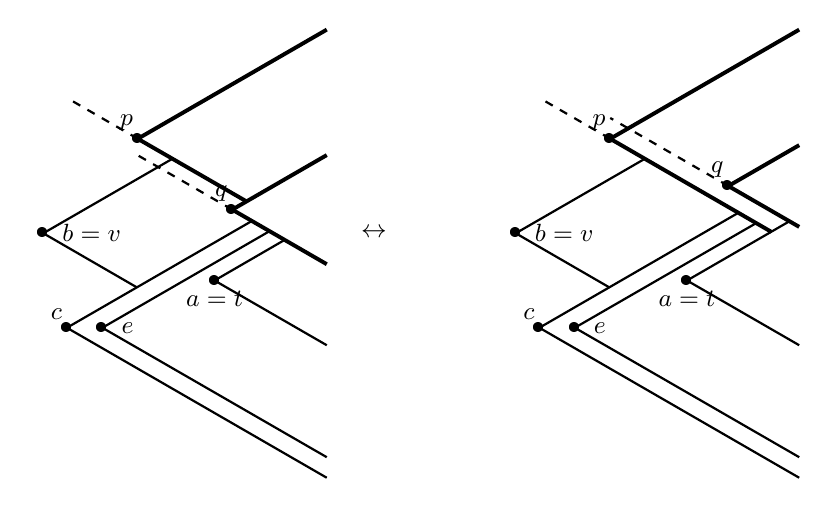
\begin{tikzpicture}[thick, scale=0.3]
        \node[label={[label distance = -3mm]160:$p$}] at
        (2.00, 4.00) {\textbullet};
        \node[label={[label distance = -3mm]160:$q$}] at
        (6.00, 1.00) {\textbullet};
        \node[label={[label distance = -2mm]270:$a = t$}] at
        (5.25, -2.00) {\textbullet};
        % \node[label={[label distance = -3mm]160:$b$}] at (-5.00, 0.00) {\textbullet};
        \node[label={[label distance = -3mm]160:$c$}] at
        (-1.00, -4.00) {\textbullet};
        \node[label={[label distance = -1mm]0:$b = v$}] at
        (-2.00, 0.00) {\textbullet};
        \node[label={[label distance = -1mm]0:$e$}] at
        (0.50, -4.00) {\textbullet};

        % q cone
        \draw[line width = 0.5mm] (6.00, 1.00) -- (10.00, -1.31);
        \draw[line width = 0.5mm] (6.00, 1.00) -- (10.00, 3.31);
        % a cone
        \draw (5.25, -2.00) -- (10.00, -4.74);
        \draw (5.25, -2.00) -- (8.22, -0.28);
        % p cone
        \draw[line width = 0.5mm] (2.00, 4.00) -- (6.60, 1.35);
        \draw[line width = 0.5mm] (2.00, 4.00) -- (10.00, 8.62);
        % c cone
        \draw (-1.00, -4.00) -- (10.00, -10.35);
        \draw (-1.00, -4.00) -- (6.83, 0.52);
        % e cone
        \draw (0.50, -4.00) -- (10.00, -9.48);
        \draw (0.50, -4.00) -- (7.58, 0.09);
        % b cone
        \draw (-2.00, 0.00) -- (1.96, -2.29);
        \draw (-2.00, 0.00) -- (3.46, 3.15);
        % b cone
        % \draw (-5.00, 0.00) -- (0.46, -3.15);
        % \draw (-5.00, 0.00) -- (10.00, 8.66);

        \draw[dashed] (2.00, 4.00) -- (-1.00, 5.73);
        \draw[dashed] (6.00, 1.00) -- (2.00, 3.30);
        \node at (12, 0) {$ \leftrightarrow$};

        \node[label={[label distance = -3mm]160:$p$}] at
        (22.00, 4.00) {\textbullet};
        \node[label={[label distance = -3mm]160:$q$}] at
        (27.00, 2.00) {\textbullet};
        \node[label={[label distance = -2mm]270:$a = t$}] at
        (25.25, -2.00) {\textbullet};
        % \node[label={[label distance = -3mm]160:$b$}] at (15.00, 0.00) {\textbullet};
        \node[label={[label distance = -3mm]160:$c$}] at
        (19.00, -4.00) {\textbullet};
        \node[label={[label distance = -1mm]0:$b = v$}] at
        (18.00, 0.00) {\textbullet};
        \node[label={[label distance = -1mm]0:$e$}] at
        (20.50, -4.00) {\textbullet};

        % q cone
        \draw[line width = 0.5mm] (27.00, 2.00) -- (30.00, 0.27);
        \draw[line width = 0.5mm] (27.00, 2.00) -- (30.00, 3.73);
        % a cone
        \draw (25.25, -2.00) -- (30.00, -4.74);
        \draw (25.25, -2.00) -- (29.59, 0.51);
        % p cone
        \draw[line width = 0.5mm] (22.00, 4.00) -- (28.82, 0.06);
        \draw[line width = 0.5mm] (22.00, 4.00) -- (30.00, 8.62);
        % e cone
        \draw (20.50, -4.00) -- (30.00, -9.48);
        \draw (20.50, -4.00) -- (28.18, 0.43);
        % c cone
        \draw (19.00, -4.00) -- (30.00, -10.35);
        \draw (19.00, -4.00) -- (27.43, 0.87);
        % b cone
        \draw (18.00, 0.00) -- (21.96, -2.29);
        \draw (18.00, 0.00) -- (23.46, 3.15);
        % b cone
        % \draw (15.00, 0.00) -- (20.46, -3.15);
        % \draw (15.00, 0.00) -- (30.00, 8.66);

        \draw[dashed] (22.00, 4.00) -- (19.00, 5.73);
        \draw[dashed] (27.00, 2.00) -- (22.00, 4.88);
    \end{tikzpicture}
    \caption{Da esquerda para a direita, o caso em que $p$ está em
        $\Hits_{low}(q)$, ou seja, $q$ está entrando em $\Dom(p)$. Da direita
        para a esquerda, o caso em que $q$ está em $\Cands(p)$, saindo de
        $\Dom(p)$.}
    \label{fig:parcinetico:eventoup}
\end{figure}

No caso de um evento em que ocorre uma mudança na $60^\circ$-ordem, que é a ordem dos pontos
projetados no eixo $x + 60^\circ$, vamos assumir que $p$ é o ponto que está à esquerda e acima de $q$.
O evento pode provocar a entrada ou saída do ponto $q$ de $\Cands(p)$, veja a
Figura~\ref{fig:parcinetico:eventoup}.
O Algoritmo~\ref{alg:par-cinetico:eventoup} implementa a sequência de operações referentes a este
evento.

Se $p$ está em $\Hits_{low}(q)$, ou seja, $q$ está entrando em $\Dom(p)$ como demonstrado na
Figura~\ref{fig:parcinetico:eventoup} da esquerda para direita, então a troca na $60^\circ$-ordem
afetará o ponto $v$ tal que $q$ está em $\Cands(v)$.
A mudança também afetará todos os pontos que estão à esquerda de $p$ e estão em $\Hits_{up}(q)$,
incluindo o ponto $t$ em $\Hits_{up}(q)$ mais à esquerda que está à direita de $p$.
Se esse ponto $t$ não existe, buscamos pelo ponto $t$ tal que $q$ está em $\Hits_{low}(t)$.
Buscamos por $t$ para que possamos remover o ponto $p$ de $\Hits_{low}(q)$ e o inseri-lo em
$\Hits_{low}(t)$.
As operações necessárias para corrigir as estruturas envolvidas estão descritas no
Algoritmo~\ref{alg:par-cinetico:eventoupcaso1}.
Se $p$ não está em $\Hits_{low}(q)$ não haverão mudanças.

\begin{algorithm}[H]
    \caption[Algoritmo \textsc{upEventLeft} do par mais próximo cinético]{Função \textsc{upEventLeft}.}
    \label{alg:par-cinetico:eventoupcaso1}
    \begin{algorithmic}[1]
        \Function{upEventLeft}{$p, q, dir$}
            \State $v \leftarrow \Call{owner}{q.cands(dir)}$ \Comment{$q \in \Cands(v)$}
            \If{$v \neq \nnull$}
                \State \Call{delete}{$q, Cands(v, dir)$}
            \EndIf
            \State \Call{insert}{$q, Cands(p, dir)$}
            \State $t \leftarrow \Call{successor}{p, \Hits_{up}(q, dir), H}$
            \If{$t = \nnull$}
                \State $t \leftarrow \Call{owner}{q.hitsLow(dir)}$ \Comment{$q \in \Hits_{low}(t)$}
            \EndIf
            \State $newHits \leftarrow \Call{split}{\nnull, t, \Hits_{up}(q, dir)}$ \Comment{anteriores a $t$ em $\Hits_{up}(q)$}
            \State $\Call{join}{\Hits_{up}(p, dir), newHits}$
            \State $\Call{delete}{p, \Hits_{low}(q, dir)}$
            \If{$t \neq \nnull$}
                \State \Call{insert}{$p, \Hits_{low}(t, dir)$}
            \EndIf
        \EndFunction
    \end{algorithmic}
\end{algorithm}

\begin{algorithm}[H]
    \caption[Algoritmo \textsc{upEventRight} do par mais próximo cinético]{Função \textsc{upEventRight}.}
    \label{alg:par-cinetico:eventoupcaso2}
    \begin{algorithmic}[1]
        \Function{upEventRight}{$p, q, dir$}
            \State $t \leftarrow \Call{owner}{p.hitsLow(dir)}$ \Comment{$p \in \Hits_{low}(t)$}
            \If{$t \neq \nnull$}
                \State \Call{delete}{$p, \Hits_{low}(t, dir)$}
            \EndIf
            \State $\Call{insert}{p, \Hits_{low}(q, dir)}$
            \State $v \leftarrow \Call{predecessor}{q, \Hits_{up}(p, dir), U}$
            \If{$v = \nnull$}
                \State $v \leftarrow \Call{owner}{p.cands(dir)}$ \Comment{$p \in \Cands(v)$}
            \EndIf
            \State $newHits \leftarrow \Call{split}{v, \nnull, \Hits_{up}(p,dir)}$
            \Comment{posteriores a $v$ em $\Hits_{up}(p)$}
            \State $\Call{join}{newHits, \Hits_{up}(q, dir)}$
            \State \Call{delete}{$q, Cands(p, dir)$}
            \If{$v \neq \nnull$}
                \State \Call{insert}{$q, Cands(v, dir)$}
            \EndIf
        \EndFunction
    \end{algorithmic}
\end{algorithm}

Se $q$ está em $\Cands(p)$, ou seja, $q$ está saindo de $\Dom(p)$ como demonstrado na
Figura~\ref{fig:parcinetico:eventoup} da direita para a esquerda, as mudanças serão similares,
porém reversas ao outro caso, como demonstrado no Algoritmo~\ref{alg:par-cinetico:eventoupcaso2}.

\begin{figure}[h]
    \centering
    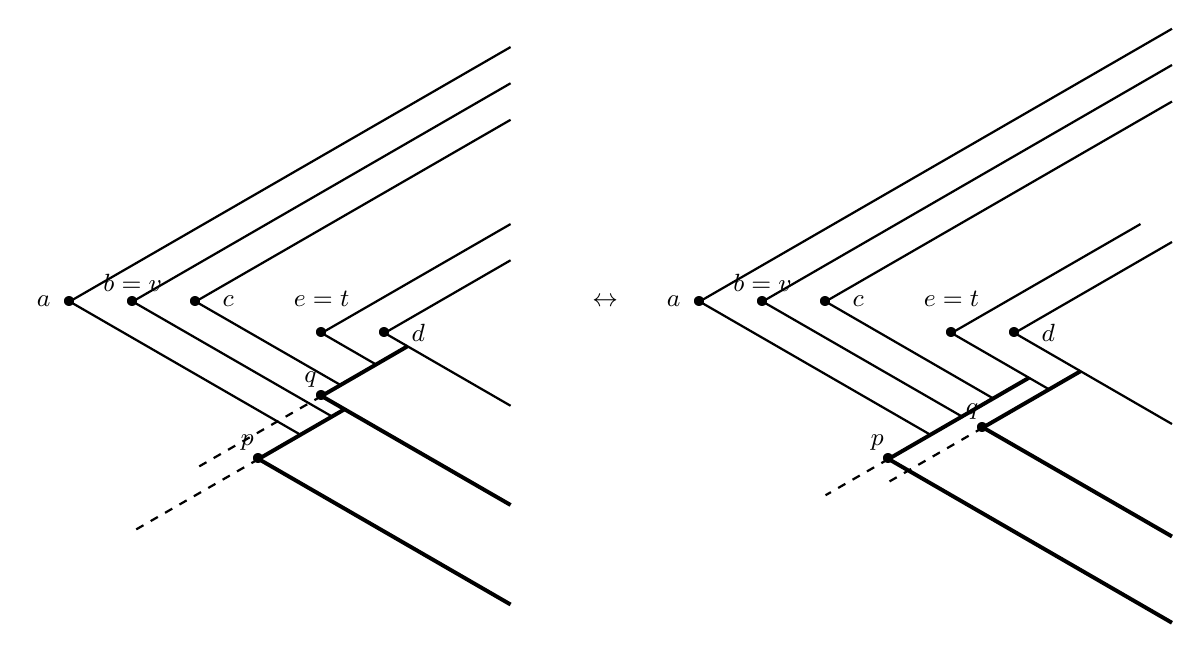
\begin{tikzpicture}[thick, scale=0.4]
        \node[label={[label distance = -3mm]160:$p$}] at
            (6.00, 0.00) {\textbullet};
        \node[label={[label distance = -3mm]160:$q$}] at
            (8.00, 2.00) {\textbullet};
        \node[label={[label distance = -1mm]180:$a$}] at
            (0.00, 5.00) {\textbullet};
        \node[label={[label distance = -2mm]90:$b = v$}] at
            (2.00, 5.00) {\textbullet};
        \node[label={[label distance = 0mm]0:$c$}] at
            (4.00, 5.00) {\textbullet};
        \node[label={[label distance = 0mm]0:$d$}] at
            (10.00, 4.00) {\textbullet};
        \node[label={[label distance = 0mm]90:$e = t$}] at
            (8.00, 4.00) {\textbullet};

        % d cone
        \draw (10.00, 4.00) -- (14.00, 1.69);
        \draw (10.00, 4.00) -- (14.00, 6.31);
        % q cone
        \draw[dashed] (8.00, 2.00) -- (4.00, -0.30);
        \draw[line width = 0.5mm] (8.00, 2.00) -- (14.00, -1.46);
        \draw[line width = 0.5mm] (8.00, 2.00) -- (10.73, 3.58);
        % e cone
        \draw (8.00, 4.00) -- (9.73, 3.00);
        \draw (8.00, 4.00) -- (14.00, 7.46);
        % p cone
        \draw[dashed] (6.00, 0.00) -- (2.00, -2.30);
        \draw[line width = 0.5mm] (6.00, 0.00) -- (14.00, -4.62);
        \draw[line width = 0.5mm] (6.00, 0.00) -- (8.73, 1.58);
        % c cone
        \draw (4.00, 5.00) -- (8.60, 2.35);
        \draw (4.00, 5.00) -- (14.00, 10.77);
        % b cone
        \draw (2.00, 5.00) -- (8.33, 1.35);
        \draw (2.00, 5.00) -- (14.00, 11.93);
        % a cone
        \draw (0.00, 5.00) -- (7.33, 0.77);
        \draw (0.00, 5.00) -- (14.00, 13.08);

        \node at (17, 5) {$ \leftrightarrow$};

        \node[label={[label distance = -3mm]160:$p$}] at
            (26.00, 0.00) {\textbullet};
        \node[label={[label distance = -3mm]160:$q$}] at
            (29.00, 1.00) {\textbullet};
        \node[label={[label distance = -1mm]180:$a$}] at
            (20.00, 5.00) {\textbullet};
        \node[label={[label distance = -2mm]90:$b = v$}] at
            (22.00, 5.00) {\textbullet};
        \node[label={[label distance = 0mm]0:$c$}] at
            (24.00, 5.00) {\textbullet};
        \node[label={[label distance = 0mm]0:$d$}] at
            (30.00, 4.00) {\textbullet};
        \node[label={[label distance = 0mm]90:$e = t$}] at
            (28.00, 4.00) {\textbullet};

        % d cone
        \draw (30.00, 4.00) -- (35.00, 1.11);
        \draw (30.00, 4.00) -- (35.00, 6.89);
        % q cone
        \draw[dashed] (29.00, 1.00) -- (26.00, -0.73);
        \draw[line width = 0.5mm] (29.00, 1.00) -- (35.00, -2.46);
        \draw[line width = 0.5mm] (29.00, 1.00) -- (32.10, 2.79);
        % e cone
        \draw (28.00, 4.00) -- (31.10, 2.21);
        \draw (28.00, 4.00) -- (34.00, 7.46);
        % p cone
        \draw[dashed] (26.00, 0.00) -- (24.00, -1.15);
        \draw[line width = 0.5mm] (26.00, 0.00) -- (35.00, -5.20);
        \draw[line width = 0.5mm] (26.00, 0.00) -- (30.46, 2.58);
        % c cone
        \draw (24.00, 5.00) -- (29.33, 1.92);
        \draw (24.00, 5.00) -- (35.00, 11.35);
        % b cone
        \draw (22.00, 5.00) -- (28.33, 1.35);
        \draw (22.00, 5.00) -- (35.00, 12.51);
        % a cone
        \draw (20.00, 5.00) -- (27.33, 0.77);
        \draw (20.00, 5.00) -- (35.00, 13.66);
    \end{tikzpicture}
    \caption{Da esquerda para direita, o caso em que
    $p$ está em $\Hits_{up}(q)$, ou seja, $q$ está
    entrando em $\Dom(p)$. Da direita para esquerda,
    o caso em que $q$ está em $\Cands(p)$, saindo
    de $\Dom(p)$.}
    \label{fig:parcinetico:eventodown}
\end{figure}

Um evento em que ocorre uma mudança na $-60^\circ$-ordem, a ordem dos pontos projetados no eixo $x
- 60^\circ$, é simétrico a um evento na $60^\circ$-ordem.
Os pontos envolvidos no evento serão $p$e $q$ e vamos assumir que $p$ é o ponto mais à esquerda e
abaixo de $q$.
O evento pode provocar a entrada ou saída do ponto $q$ de $\Cands(p)$, veja a
Figura~\ref{fig:parcinetico:eventodown}.
O Algoritmo~\ref{alg:par-cinetico:eventodown} implementa a sequência de operações referentes a esse
evento.

\begin{figure}[h]
    \centering
    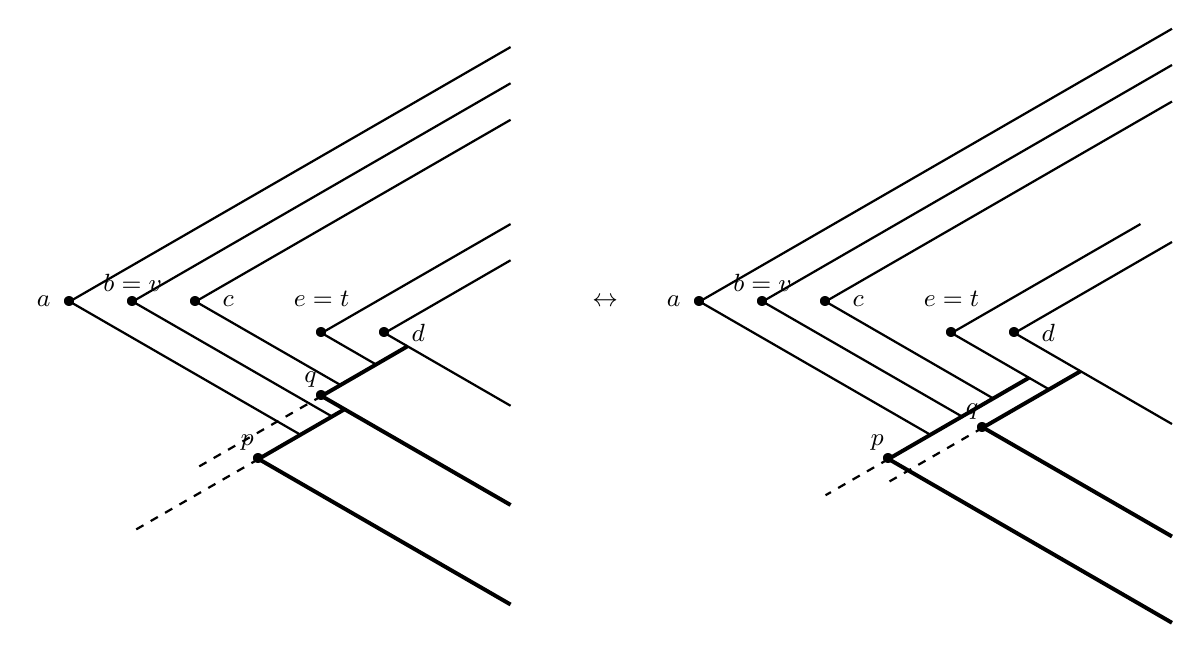
\begin{tikzpicture}[thick, scale=0.4]
        \node[label={[label distance = -3mm]160:$p$}] at
            (6.00, 0.00) {\textbullet};
        \node[label={[label distance = -3mm]160:$q$}] at
            (8.00, 2.00) {\textbullet};
        \node[label={[label distance = -1mm]180:$a$}] at
            (0.00, 5.00) {\textbullet};
        \node[label={[label distance = -2mm]90:$b = v$}] at
            (2.00, 5.00) {\textbullet};
        \node[label={[label distance = 0mm]0:$c$}] at
            (4.00, 5.00) {\textbullet};
        \node[label={[label distance = 0mm]0:$d$}] at
            (10.00, 4.00) {\textbullet};
        \node[label={[label distance = 0mm]90:$e = t$}] at
            (8.00, 4.00) {\textbullet};

        % d cone
        \draw (10.00, 4.00) -- (14.00, 1.69);
        \draw (10.00, 4.00) -- (14.00, 6.31);
        % q cone
        \draw[dashed] (8.00, 2.00) -- (4.00, -0.30);
        \draw[line width = 0.5mm] (8.00, 2.00) -- (14.00, -1.46);
        \draw[line width = 0.5mm] (8.00, 2.00) -- (10.73, 3.58);
        % e cone
        \draw (8.00, 4.00) -- (9.73, 3.00);
        \draw (8.00, 4.00) -- (14.00, 7.46);
        % p cone
        \draw[dashed] (6.00, 0.00) -- (2.00, -2.30);
        \draw[line width = 0.5mm] (6.00, 0.00) -- (14.00, -4.62);
        \draw[line width = 0.5mm] (6.00, 0.00) -- (8.73, 1.58);
        % c cone
        \draw (4.00, 5.00) -- (8.60, 2.35);
        \draw (4.00, 5.00) -- (14.00, 10.77);
        % b cone
        \draw (2.00, 5.00) -- (8.33, 1.35);
        \draw (2.00, 5.00) -- (14.00, 11.93);
        % a cone
        \draw (0.00, 5.00) -- (7.33, 0.77);
        \draw (0.00, 5.00) -- (14.00, 13.08);

        \node at (17, 5) {$ \leftrightarrow$};

        \node[label={[label distance = -3mm]160:$p$}] at
            (26.00, 0.00) {\textbullet};
        \node[label={[label distance = -3mm]160:$q$}] at
            (29.00, 1.00) {\textbullet};
        \node[label={[label distance = -1mm]180:$a$}] at
            (20.00, 5.00) {\textbullet};
        \node[label={[label distance = -2mm]90:$b = v$}] at
            (22.00, 5.00) {\textbullet};
        \node[label={[label distance = 0mm]0:$c$}] at
            (24.00, 5.00) {\textbullet};
        \node[label={[label distance = 0mm]0:$d$}] at
            (30.00, 4.00) {\textbullet};
        \node[label={[label distance = 0mm]90:$e = t$}] at
            (28.00, 4.00) {\textbullet};

        % d cone
        \draw (30.00, 4.00) -- (35.00, 1.11);
        \draw (30.00, 4.00) -- (35.00, 6.89);
        % q cone
        \draw[dashed] (29.00, 1.00) -- (26.00, -0.73);
        \draw[line width = 0.5mm] (29.00, 1.00) -- (35.00, -2.46);
        \draw[line width = 0.5mm] (29.00, 1.00) -- (32.10, 2.79);
        % e cone
        \draw (28.00, 4.00) -- (31.10, 2.21);
        \draw (28.00, 4.00) -- (34.00, 7.46);
        % p cone
        \draw[dashed] (26.00, 0.00) -- (24.00, -1.15);
        \draw[line width = 0.5mm] (26.00, 0.00) -- (35.00, -5.20);
        \draw[line width = 0.5mm] (26.00, 0.00) -- (30.46, 2.58);
        % c cone
        \draw (24.00, 5.00) -- (29.33, 1.92);
        \draw (24.00, 5.00) -- (35.00, 11.35);
        % b cone
        \draw (22.00, 5.00) -- (28.33, 1.35);
        \draw (22.00, 5.00) -- (35.00, 12.51);
        % a cone
        \draw (20.00, 5.00) -- (27.33, 0.77);
        \draw (20.00, 5.00) -- (35.00, 13.66);
    \end{tikzpicture}
    \caption{Da esquerda para direita, o caso em que
    $p$ está em $\Hits_{up}(q)$, ou seja, $q$ está
    entrando em $\Dom(p)$. Da direita para esquerda,
    o caso em que $q$ está em $\Cands(p)$, saindo
    de $\Dom(p)$.}
    \label{fig:parcinetico:eventodown}
\end{figure}

Se $p$ está em $\Hits_{up}(q)$ ($q$ está entrando em $Dom(p)$), como demonstrado na
Figura~\ref{fig:parcinetico:eventodown}, então a troca na $-60^\circ$-ordem afetará o ponto $v$ tal
que $q$ está em $\Cands(v)$.
Além disso, afetará $\Cands(p)$, todos os pontos que estão à esquerda de $p$ e estão em
$\Hits_{low}(q)$, incluindo o ponto $t$ em $\Hits_{low}(q)$ mais à esquerda que está a
direita de $p$.
Se não existe ponto que satisfaça essas condições, então buscamos pelo ponto $t$ tal que $q$ está
em $\Hits_{up}(t)$.
Buscamos por $t$ porque precisamos remover o ponto $p$ de $\Hits_{up}(q)$ e o inserimos em
$\Hits_{up}(t)$.
Se $p$ não está em $\Hits_{up}(q)$ não haverão mudanças.
As operações necessárias para corrigir as estruturas envolvidas estão descritas no
Algoritmo~\ref{alg:par-cinetico:eventoupcaso1}.

\begin{algorithm}[H]
    \caption[Algoritmo \textsc{downEventLeft} do par mais próximo cinético]{Função downEventLeft.} \label{alg:par-cinetico:eventodowncaso1}
    \begin{algorithmic}[1]
        \Function{downEventLeft}{$p, q, dir$}
            \State $v \leftarrow \Call{owner}{q.cands(dir)}$
            \If{$v \neq \nnull$}
                \State \Call{delete}{$q, Cands(v, dir)$}
            \EndIf
            \State \Call{insert}{$q, Cands(p, dir)$}
            \State $t \leftarrow \Call{successor}{p, \Hits_{low}(q, dir), H}$
            \If{$t = \nnull$}
                \State $t \leftarrow \Call{owner}{q.hitsUp(dir)}$
            \EndIf
            \State $newHits \leftarrow \Call{split}{\nnull, t, \Hits_{low}(q, dir)}$
            \State $\Call{join}{\Hits_{low}(p, dir), newHits}$
            \State $\Call{delete}{p, \Hits_{up}(q, dir)}$
            \If{$t \neq \nnull$}
                \State \Call{insert}{$p, \Hits_{up}(t, dir)$}
            \EndIf
        \EndFunction
    \end{algorithmic}
\end{algorithm}

Se $q$ está em $\Cands(p)$ ($q$ está saindo de $Dom(p)$), como demonstrado na
Figura~\ref{fig:parcinetico:eventodown}, as mudanças serão similares, porém reversas ao outro
caso, como demonstrado no Algoritmo~\ref{alg:par-cinetico:eventodowncaso2}.

\begin{algorithm}[H]
    \caption{Função downEventRight.} \label{alg:par-cinetico:eventodowncaso2}
    \begin{algorithmic}[1]
        \Function{downEventRight}{$p, q, dir$}
            \State $t \leftarrow \Call{owner}{p.hitsUp(dir)}$
            \If{$t \neq \nnull$}
                \State \Call{delete}{$p, \Hits_{up}(t, dir)$}
            \EndIf
            \State $\Call{insert}{p, \Hits_{up}(q, dir)}$
            \State $v \leftarrow \Call{predecessor}{q, \Hits_{low}(p, dir), D}$
            \If{$v = \nnull$}
                \State $v \leftarrow \Call{owner}{p.cands(dir)}$
            \EndIf
            \State $newHits \leftarrow \Call{split}{v, \nnull, \Hits_{low}(p,dir)}$
            \State $\Call{join}{newHits, \Hits_{low}(q, dir)}$
            \State \Call{delete}{$q, Cands(p, dir)$}
            \If{$v \neq \nnull$}
                \State \Call{insert}{$q, Cands(v, dir)$}
            \EndIf
        \EndFunction
    \end{algorithmic}
\end{algorithm}

\FloatBarrier

\subsection{Análise de desempenho}\label{subsec:par:analise-de-desempenho}

As análises de desempenho aqui foram extraídas de~\cite{eduardo}.

A estrutura de dados cinética para manter um par de pontos mais próximo é uma estrutura
\textit{responsiva}, pois o custo de processar um certificado é $O(\lg{n})$, onde $n$ é o número
de pontos.
O custo de processar um certificado é o custo de realizar as trocas necessárias nas listas
ordenadas, o que consome tempo $O(\lg{n})$.
Além disso também há o custo de corrigir as árvores $\Cands$, $\Hits_{low}$, $\Hits_{up}$, o
torneio e os certificados associados.
Mas, essas operações são realizadas em sequência, consumindo um custo também de $O(\lg{n})$.

A estrutura é \textit{eficiente}, pois a razão entre o total de eventos e os eventos
\textit{externos}, isto é, as trocas de par mais próximo, de acordo com~\cite{eduardo}, é
$O(\epsilon \lg{n})$, resultando em uma estrutura eficiente.

A estrutura é \textit{compacta}, pois teremos $O(n)$ certificados na fila de prioridades
associados a mudanças nas listas ordenadas e $O(n)$ certificados do torneio cinético, resultando
em $O(n)$ certificados na fila com prioridades num determinado instante.

A estrutura é \textit{local}, pois um ponto pode estar envolvido em até seis certificados das
listas ordenadas, sendo dois para cada uma das ordenações, e pode estar envolvido em até
$O(\lg{n})$ certificados no torneio.
